\chapter{Wyniki eksperymentalne}\label{ch:exp}
\thispagestyle{chapterBeginStyle}





W~tym rozdziale pochylimy się nad eksperymentalnymi wynikami, które uzyskaliśmy dla wybranych przypadków testowych.
Jako że problem \textsc{Recoverable Robust Incremental Minimum Spanning Tree} sam składa się z~wielu podproblemów, część eksperymentalną zaczniemy właśnie od nich, by przekonać się między innymi o~różnicach, które wynikają z~zastosowania różnych algorytmów do rozwiązywania tych samych instancji problemu.
W~rozdziale \ref{ch:binaryIncMST} przedstawialiśmy dwa różne podejścia do problemu \textsc{Incremental Minimum Spanning Tree}, nie mówiąc już o~rozwiązaniu, które zaproponowaliśmy pod koniec omawiania zagadnień związanych z~programowaniem liniowym~--- porównamy eksperymentalnie czasy działania dwóch pierwszych.
Jak się okaże, czas, po którym dowolny z~przytoczonych przez nas modeli programowania liniowego/całkowitoliczbowego zwraca optymalne rozwiązanie, jest zbyt duży, by jego porównywanie z~poprzednimi dwoma algorytmami miało dla nas jakąkolwiek wartość (zobacz wykresy \ref{fig:imst1:a} oraz \ref{fig:imst1:a}).
W~przypadku problemu adwersarza, który również jest częścią składową dla \textsc{Recoverable Robust Incremental Minimum Spanning Tree}, będziemy chcieli przekonać się, czy podział zadań na osobne wątki (tak jak to sugerowaliśmy w~rozdziale \ref{ch:minmax}) rzeczywiście jest dla nas opłacalny.
Wreszcie na końcu będziemy chcieli sprawdzić, jak dla różnych instancji grafów zachowuje się, przedstawiony w~poprzednim rozdziale, algorytm \textsc{Tabu Search} dla szerokiej gamy konfiguracji jego parametrów.




\section{Środowisko testowe}




O ile dla samego algorytmu \textsc{Tabu Search} nie jesteśmy zainteresowani jego rzeczywistą złożonością obliczeniową (wiemy, że algorytm działa w~czasie wielomianowym, co automatycznie czyni go szybszym od wszelkich innych prób dokładnego rozwiązania \textsc{NP}-trudnego problemu, jakim jest \textsc{Recoverable Robust Incremental Minimum Spanning Tree}), tak w~przypadku algorytmów przez nas zaproponowanych, służących do rozwiązywania problemów minimalnego drzewa rozpinającego w~wersji \textsc{Incremental} jak i~problemu adwersarza, będziemy chcieli uzyskać nadające się do interpretacji wyniki.
W~związku z~tym nasze wszystkie eksperymenty będziemy przeprowadzać na, użyczonym do tego celu, serwerze Politechniki Wrocławskiej o~nazwie \textsc{Otryt}, wspieranego przez $80$ jednostek \textsc{Intel\textsuperscript{\textregistered} Xeon\textsuperscript{\textregistered} CPU E7-4850 @ 2.00GHz}, zaopatrzonych w~$256$ \textsc{GB} pamięci \textsc{RAM} i~$6,3$ \textsc{TB} przestrzeni dyskowej, działającego pod kontrolą systemu operacyjnego \textsc{Linux Debian} w~wersji $7.7$.

Testy stabilności algorytmów i~inne pomniejsze testy zostały zaś wykonane na lokalnej maszynie pod kontrolą sytemu \textsc{Linux Ubuntu} w~wersji $15.10$ z~$4$ \textsc{GB} pamięci dynamicznej oraz $74$ \textsc{GB} przestrzeni dyskowej, zarządzanej przez procesor \textsc{Intel\textsuperscript{\textregistered} Core\textsuperscript{\texttrademark} i5 CPU M 540 @ 2.53GHz}.
Ze względu na różnice systemów obu środowisk, zdecydowano się na kompilowanie rozwiązań przy pomocy starszej wersji kompilatora \textsc{g++} (\textsc{4.9.2}) (gdzie pierwotnie rozwiązania były budowane przy pomocy tego narzędzia w~wersji \textsc{5.2.1}).




\section{Problem INCREMENTAL}




Wykorzystane przez nas przykłady będą głównie opierać się na jednym z~parametrów grafu, jakim jest jego gęstość~--- w~przypadku problemu \textsc{Incremental Minimum Spanning Tree} oraz wszystkich problemów pochodnych (\textsc{AIMST} oraz \textsc{RRIMST}), gdzie całość rozwiązania opiera się na wyborze takiego, które spełnia pewne określone własności względem innego rozwiązania (oryginalnego), kluczowym parametrem, decydującym w~głównej mierze o~zachowaniu się dowolnego z~przedstawianych algorytmów, jest bez wątpienia gęstość grafu, o~czym się przekonamy, analizując chociażby wykresy dotyczące algorytmu lokalnego przeszukiwania z~listą ruchów zakazanych \textsc{Tabu Search}.
Na tę chwilę wystarczy, że zauważymy, iż im większa jego gęstość, tym więcej krawędzi w~grafie, tym wyższe stopnie posiadają wierzchołki\footnote{
	Stopniem wierzchołka określamy liczbę krawędzi, z~którymi jest bezpośrednio połączony.
}, a~co za tym idzie~--- algorytm, którego zadaniem jest zwrócić najlepsze drzewo rozpinające $T^{\ast}$, które nie może się różnić od drzewa początkowego $T_{0}$ o~więcej niż $k$ krawędzi, na każdym etapie będzie musiał podejmować coraz więcej decyzji (zauważmy, że bez względu na gęstość grafu, liczba krawędzi, składających się na jego dowolne drzewo rozpinające, nie ulega zmianie, co znaczy, że wraz ze wzrostem gęstości rośnie także stosunek $\frac{\left| E \right|}{\left| T \right|}$, co oczywiście przekłada się bezpośrednio na czas działania takiego algorytmu).
Szczególnie widoczne jest to w~przypadku, gdy gęstość grafu jest na tyle mała, że sam ten fakt zaczyna ,,sugerować'' poprawne rozwiązania (to znaczy liczba krawędzi jest na tyle mała, że zbiór $\left\{ e : e \in T_{0} \right\}$, gdzie $T_{0}$ jest początkowym rozwiązaniem problemu \textsc{IMST}, zaczyna stanowić większość krawędzi w~grafie).
Na wykresach \ref{fig:imst1:a} oraz \ref{fig:imst1:c} uchwycono tą zależność, gdzie niebieskim kolorem zaznaczono wykresy podstawowego algorytmu rozwiązującego problem \textsc{IMST}, zaś druga krzywa z~pary przedstawia czas, w~jakim z~tymi samymi instancjami problemu poradził sobie algorytm, w~którym zastosowaliśmy wszystkie nasze uwagi, dotyczące możliwości poprawienia jego efektywności względem pierwszego algorytmu.

\begin{figure}[!htbp]
	\renewcommand\figurename{Wykres}
	\null\hfill
	\begin{subfigure}[b]{0.45\textwidth}
		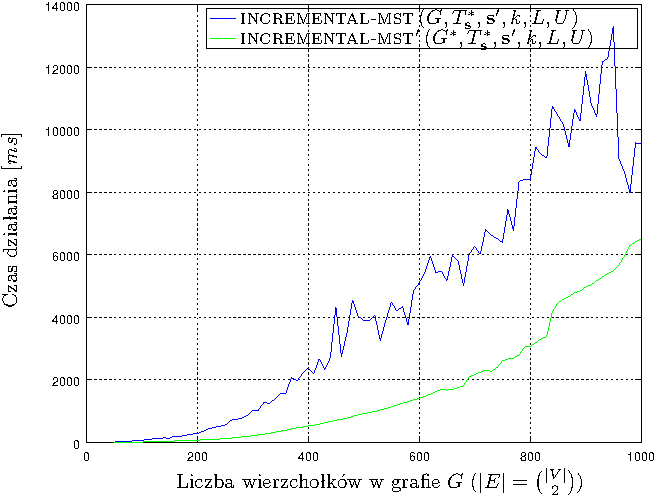
\includegraphics[width=\textwidth]{Chapter_VI/IMST1-example/IMST1_psfrag}
		\caption{}
		\label{fig:imst1:a}
	\end{subfigure}
	\hfill
	\begin{subfigure}[b]{0.45\textwidth}
		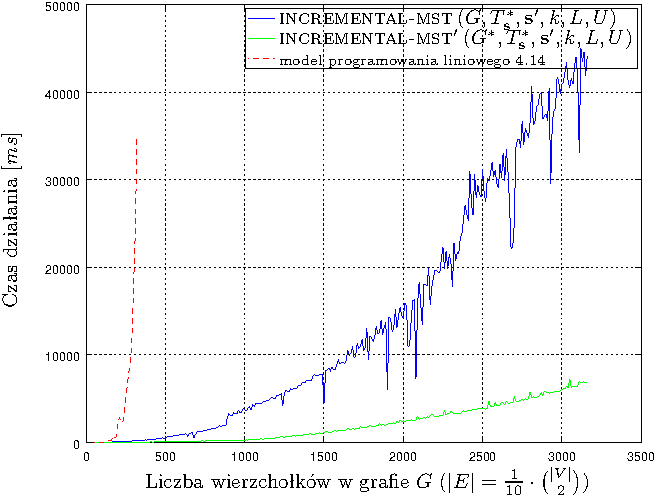
\includegraphics[width=\textwidth]{Chapter_VI/IMST3-example/IMST3_psfrag}
		\caption{}
		\label{fig:imst1:c}
	\end{subfigure}
	\hfill\null
	\caption{
		Wykres zależności czasu pracy algorytmów:
		\textbf{(a)}~$\textsc{Incremental-MST} \left( G, T^{\ast}_{\textbf{s}}, \textbf{s}^{\prime}, k, L, U \right)$ oraz \textbf{(b)}~$\textsc{Incremental-MST}^{\prime} \left( G^{\ast}, T^{\ast}_{\textbf{s}}, \textbf{s}^{\prime}, k, L, U \right)$ od liczby krawędzi w~grafie.
	}
	\label{fig:imst1}
\end{figure}

W tym drugim przypadku możemy zauważyć nie tylko większą regularność otrzymywanych rezultatów (czas, potrzebny na rozwiązywanie coraz to większych instancji problemu przez drugi z~algorytmów, jest dużo bardziej proporcjonalny do rozmiaru danych wejściowych), lecz także dużo mniejszą zależność od liczby wierzchołków w~grafie (wystarczy przywołać linie $2$--$9$ pseudokodu \ref{alg:imstbinarysearch}, opisywanego w~rozdziale \ref{ch:binaryIncMST}, aby zobaczyć, że czas wykonywania się wspomnianego fragmentu kodu stanowi znaczny ułamek całkowitego czasu działania algorytmu, gdzie dany kod jest zależny w~głównej mierze od liczby wierzchołków w~grafie\footnote{
	Całość wspomnianego kodu wykonuje się w~pętli $\left| T^{\ast}_{\textbf{s}} \setminus T^{\ast}_{\textbf{s}^{\prime}} \right|$ razy, gdzie $\left| T^{\ast}_{\textbf{s}} \right| = \left| T^{\ast}_{\textbf{s}^{\prime}} \right| = \left| V \right| - 1$.
}).
Jak możemy zauważyć w~przypadku tego algorytmu, czasy jego działania dla obu przedstawionych konfiguracji są niemal identyczne, co może świadczyć o~tym, że głównym wyznacznikiem złożoności obliczeniowej dla niego jest liczba krawędzi grafu (gdzie w~przypadku obu wykresów ich liczby są porównywalne: $\binom{1000}{2} \approx \binom{3610}{2} \cdot \frac{1}{10}$), nie zaś jego wierzchołków.
Z~analizy złożoności jednak wiemy, że czas działania opisywanego algorytmu to w~najlepszym przypadku (gdy przyjmiemy, że potrafimy rozwiązać problem minimalnego drzewa rozpinającego w~czasie $O \left( m \cdot \alpha \left( m, n \right) \right)$) czas rzędu $O \left( m \cdot \alpha  \left( m, n \right) + \log \left( n \right) \cdot n \cdot \alpha \left( n, n \right) \right)$~--- zatem przyczyny, dla której omawiany algorytm działa w~podobnym czasie zarówno dla grafu z~tysiącem wierzchołków jak i~dla takiego z~liczbą $3160$ węzłów, musimy szukać gdzie indziej.
Przyczyna takiego a~nie innego zachowania jest z~goła dużo prostsza do wytłumaczenia~--- fakt tak niewielkiej, w~porównaniu z~grafem pełnym, gęstości powoduje, że na samym już początku z~większym prawdopodobieństwem otrzymamy dwa drzewa $T^{\ast}_{\textbf{s}}$ oraz $T^{\ast}_{\textbf{s}^{\prime}}$, których część wspólna będzie większa, niż tych samych drzew odnalezionych dla grafu pełnego.
Stąd, dla niewielkiej gęstości grafu, algorytm, by znaleźć optymalne rozwiązanie problemu \textsc{Incremental Minimum Spanning Tree}, musi wykonać dużo mniejszą liczbę kroków, niż w~przypadku grafu pełnego (im większa początkowa część wspólna minimalnych drzew rozpinających $T^{\ast}_{\textbf{s}}$ oraz $T^{\ast}_{\textbf{s}^{\prime}}$, tym mniejszy zbiór $\Lambda = \left\{ c^{\prime}_{e_{i}} - c^{\prime}_{e_{j}} : e_{i} \in T^{\ast}_{\textbf{s}} \setminus T^{\ast}_{\textbf{s}^{\prime}} \; \wedge \; e_{j} \in T^{\ast}_{\textbf{s}^{\prime}} \setminus T^{\ast}_{\textbf{s}} \right\}$ do przeglądnięcia ma algorytm).
Jak widzimy, zaznaczony przerywaną czerwoną linią czas obliczeń, potrzebny do znalezienia rozwiązania dla modelu liniowego, prezentowanego w~rozdziale \ref{ch:linearprog} (patrz model \ref{mod:mst7}), jest znacznie większy, w~porównaniu do czasu działania algorytmów, które powstały w~oparciu o~ten model.

Wspominane wykresy otrzymano dla grafów, których liczba krawędzi wahała się od $50$ do $3160$, gdzie dla każdego z~nich eksperymenty zostały powtórzone $100$ razy, aby wyeliminować wpływ czynników losowych na postać generowanych wykresów.
Mimo tego musimy zdawać sobie sprawę, że wszystkie dane były generowane w~sposób losowy~--- ze względu na charakterystykę rozpatrywanego problemu nie było zatem możliwe zapewnienie większej skali podobieństwa pomiędzy kolejnymi instancjami grafu, niż przedstawiono na wykresach (zdecydowano się za parametr $k$ przyjąć wartość wprost proporcjonalną do liczy krawędzi, składających się na drzewo rozpinające grafu).




\section{Problem adwersarza}




Kolejnym problemem stojącym na drodze do problemu odpornej optymalizacji z~możliwością poprawy, jest problem adwersarza, który omawialiśmy w~rozdziale \ref{ch:minmax} (patrz podrozdział \ref{sec:adv})~--- wspomnieliśmy wtedy tylko o~tym, że algorytm rozwiązujący dane zagadnienie, ze względu na charakterystykę matematycznego sformułowania opisującego problem ($\max_{\textbf{s}^{\prime} \in S} \min_{\textbf{y} \in X^{k}_{\textbf{x}}} v \left( \textbf{y}, \textbf{s}^{\prime} \right)$), może zostać zaimplementowany z~wykorzystaniem mechanizmu wątków, które umożliwią wykonywanie się obliczeń dla zawartych w~nim podproblemów ($\min_{\textbf{y} \in X^{k}_{\textbf{x}}} v \left( \textbf{y}, \textbf{s}^{\prime} \right)$) w~tym samym czasie, niezależnie od pozostałych (jeżeli liczba dostępnych wątków w~odniesieniu do liczby scenariuszy jest wystarczająco duża i~co najmniej równa liczbie tych drugich). 

\begin{figure}[!htbp]
	\renewcommand\figurename{Wykres}
	\null\hfill
	\begin{subfigure}[b]{0.45\textwidth}
		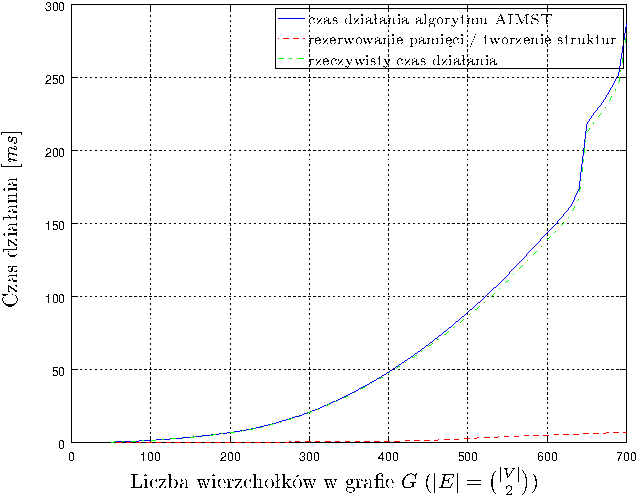
\includegraphics[width=\textwidth]{Chapter_VI/AIMST1-example/AIMST1_psfrag}
		\caption{}
		\label{fig:aimst1:a}
	\end{subfigure}
	\hfill
	\begin{subfigure}[b]{0.45\textwidth}
		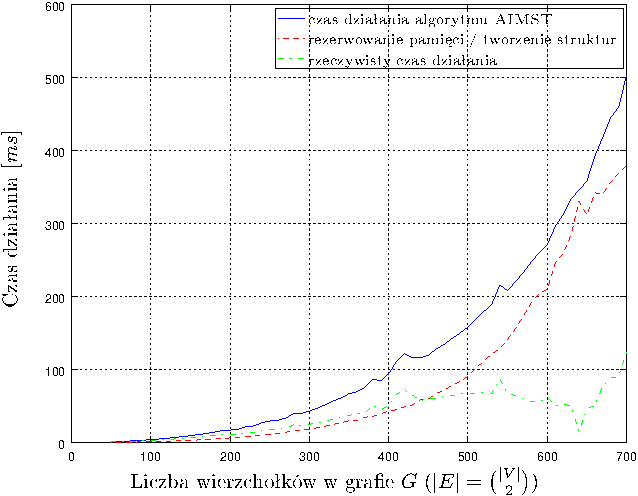
\includegraphics[width=\textwidth]{Chapter_VI/AIMST2-example/AIMST2_psfrag}
		\caption{}
		\label{fig:aimst1:b}
	\end{subfigure}
	\hfill\null
	\caption{
		Czas działania algorytmu rozwiązującego problem adwersarza dla $70$ scenariuszy, wygenerowanych dla grafu pełnego.
		Na każdym z~wykresów przedstawiono czas działania algorytmu (niebieska linia), na który składają się takie procesy jak: alokacja pamięci oraz tworzenie wymaganych struktur danych (czerwona przerywana linia) oraz sam proces obliczeń, gdzie przebieg tego ostatniego został zaznaczony przerywaną linią zieloną.
		 \textbf{(a)}~Czas działania algorytmu w~przypadku uruchomienia go bez wsparcia dla wielu wątków~--- algorytm sekwencyjnie wykonuje obliczenia dla każdego z~$70$ scenariuszy,
		 \textbf{(b)}~w~odróżnieniu od sytuacji na drugim wykresie, gdzie zezwolono algorytmowi na wykorzystanie pełnej równoległości, gdzie każdy z~$70$ scenariuszy może być rozpatrywany niezależnie.
	}
	\label{fig:aimst1}
\end{figure}

Na wykresach \ref{fig:aimst1:a} oraz \ref{fig:aimst1:b} przedstawiono dwa sposoby podejścia do rozpatrywanego problemu~--- na drugim z~nich widzimy algorytm z~, zaproponowanym przez nas, wykorzystaniem wielu wątków procesorów, zaś pierwszy ukazuje czas działania tego samego algorytmu, tyle że pracującego sekwencyjnie.
Co zaskakujące, czas działania tego ostatniego jest dużo lepszy niż dla algorytmu wykorzystującego wielowątkowość~--- wytłumaczenie tego zjawiska jest jednak oczywiste, jeżeli weźmiemy pod uwagę fakt, iż aby możliwe były równoległe obliczenia na grafie, gdzie zmieniają one jego właściwości (koszty krawędzi), muszą one być wykonywane na niezależnych od siebie obiektach, co już na samym początku wydłuża czas działania całego algorytmu o~czas potrzebny na $K$-krotne skopiowanie całej struktury grafu, gdzie $K$ to liczba scenariuszy adwersarza. 
W~rozpatrywanym przypadku celowo wykorzystaliśmy graf pełny, aby spotęgować ten negatywny efekt rozbicia pracy algorytmu na wiele wątków.
W~grafie pełnym liczbę krawędzi szacujemy na $\left| V \right|^{2}$, co stanowi niemal najbardziej znaczący składnik złożoności algorytmu \textsc{IMST}, jaką otrzymaliśmy pod koniec rozdziału \ref{ch:binaryIncMST}~--- $O \left( m \cdot \alpha  \left( m, n \right) + \log \left( n \right) \cdot n \cdot \alpha \left( n, n \right) \right)$, gdzie $m \cdot \alpha  \left( m, n \right) \approx m$. 
W~przypadku gdy nie bralibyśmy pod uwagę czasu potrzebnego na te operacje (czas ten zaznaczyliśmy czerwonym kolorem na wykresach \ref{fig:aimst1:a} oraz \ref{fig:aimst1:b}), bądź rozwiązali problem w~inny sposób (np. zbudowali nasze struktury od podstaw z~myślą o~wielowątkowości, co pozwoliłoby nam przenieść znaczną część obliczeń, związanych z~powielaniem struktur danych, na równoległe wątki\footnote{
	Musielibyśmy rozwiązać problem jednoczesnego dostępu do danych oryginalnego grafu, gdyż prezentowane przykłady wykorzystują struktury, które w~takich przypadkach wymuszają sekwencyjne odczytywanie danych przez każdy wątek po kolei, co oczywiście znacznie osłabia potęgę, drzemiącą w~podejściu równoległym do problemu.
}), w~oczywisty sposób drugi z~przedstawionych wariantów okazałby się bezkonkurencyjny (rzeczywisty czas działania, dla którego nie braliśmy pod uwagę czasu poświęconego na organizowanie danych dla algorytmu, zaznaczyliśmy na wykresach kolorem zielonym).




\section{Tabu Search}




Tak jak to miało miejsce wyżej, także dla problemu odpornej optymalizacji dyskretnej z~możliwością poprawy dla minimalnego drzewa rozpinającego przy wykorzystaniu algorytmu lokalnego przeszukiwania, gęstość grafu będzie miała niebagatelne znaczenie dla przebiegu całego procesu obliczeniowego.
Jak mogliśmy zaobserwować w~poprzedniej części, w~przypadku grafów pełnych pomysł zrównoleglania okazał się bardzo niekorzystny ze względu na konieczność wielokrotnego przekopiowywania dużej ilości danych (zwłaszcza liczby krawędzi, kwadratowej w~stosunku do $V$), w~celu oddzielenia od siebie obliczeń.

\begin{figure}[!htbp]
	\renewcommand\figurename{Wykres}
	\null\hfill
	\begin{subfigure}[b]{0.45\textwidth}
		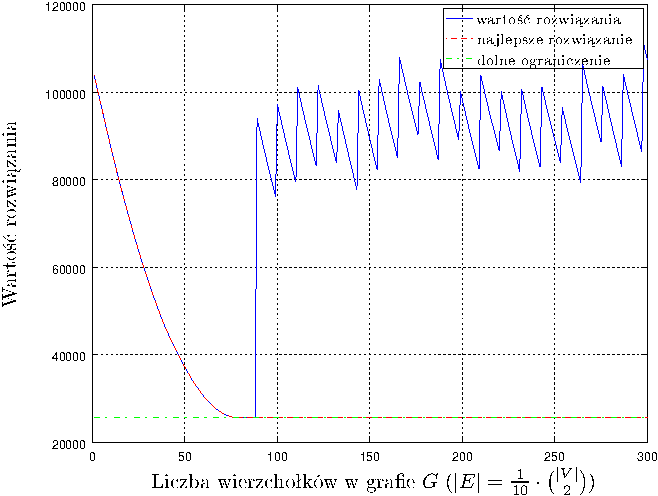
\includegraphics[width=\textwidth]{Chapter_VI/RRIMST1-example/RRIMST1_psfrag}
		\caption{}
		\label{fig:rrimst1:a}
	\end{subfigure}
	\hfill
	\begin{subfigure}[b]{0.45\textwidth}
		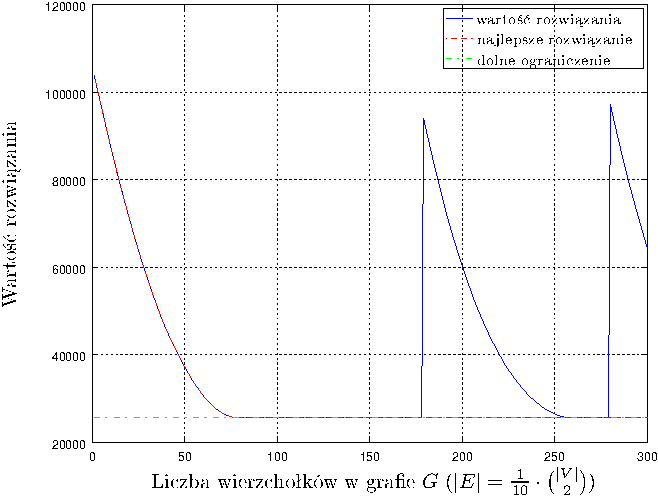
\includegraphics[width=\textwidth]{Chapter_VI/RRIMST2-example/RRIMST2_psfrag}
		\caption{}
		\label{fig:rrimst1:b}
	\end{subfigure}
	\hfill\null
	\caption{
		Wartości rozwiązań zwracane przez algorytm \textsc{Tabu Search} dla grafu o~$100$ wierzchołkach, $495$ krawędziach (gęstość grafu $q = \frac{1}{10}$), dla parametru $k = 10$, współczynników funkcji oceny ruchu (patrz \ref{eq:moveValue}) $\alpha_{1} = \alpha_{2} = \alpha_{3} = \alpha_{4} = \alpha_{5} = \frac{1}{2}$.
		Długość kadencji każdego z~elementów na liście ruchów zabronionych wynosiła $20$ iteracji, gdzie po \textbf{(a)}~$10$, \textbf{(b)}~$60$ iteracjach, w~przypadku braku polepszenia wartości dla najlepszego do tej pory znalezionego rozwiązania, algorytm porzucał obecnie badaną ścieżkę, rozpoczynając poszukiwanie rozwiązań w~innym obszarze ich przestrzeni.
	}
\end{figure}

\begin{figure}[!htbp]
	\renewcommand\figurename{Wykres}
	\ContinuedFloat
	\null\hfill
	\begin{subfigure}[b]{0.45\textwidth}
		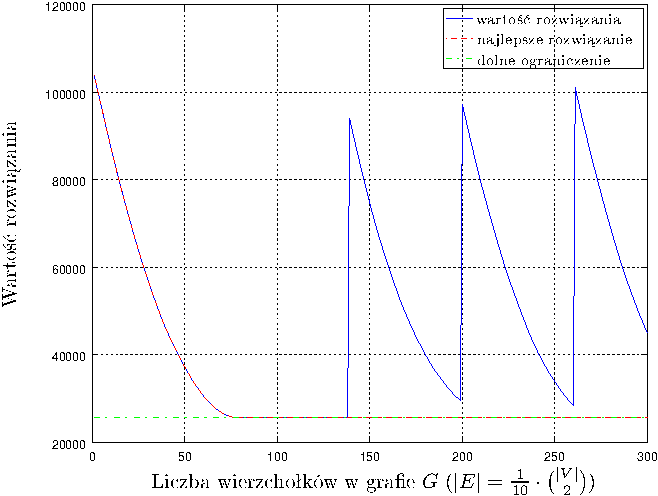
\includegraphics[width=\textwidth]{Chapter_VI/RRIMST3-example/RRIMST3_psfrag}
		\caption{}
		\label{fig:rrimst1:c}
	\end{subfigure}
	\hfill
	\begin{subfigure}[b]{0.45\textwidth}
		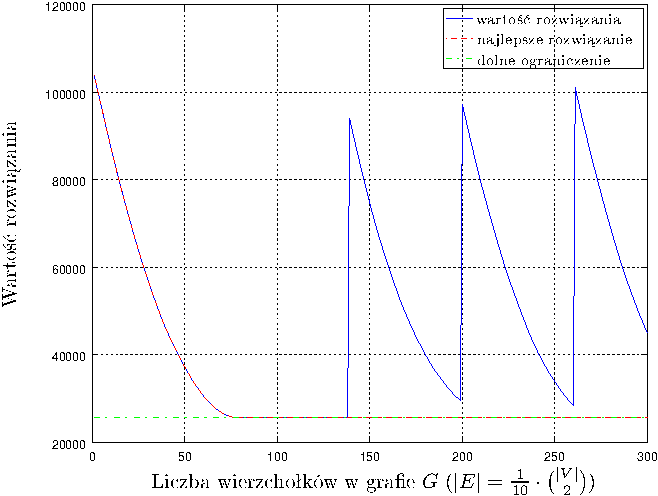
\includegraphics[width=\textwidth]{Chapter_VI/RRIMST4-example/RRIMST4_psfrag}
		\caption{}
		\label{fig:rrimst1:d}
	\end{subfigure}
	\hfill\null
	\caption{
		Wartości rozwiązań zwracane przez algorytm \textsc{Tabu Search} dla grafu o~$100$ wierzchołkach, $495$ krawędziach (gęstość grafu $q = \frac{1}{10}$), dla parametru $k = 10$, współczynników funkcji oceny ruchu (patrz \ref{eq:moveValue}): $\alpha_{1} = \alpha_{4} = \alpha_{5} = \frac{1}{10}$ oraz $\alpha_{2} = \alpha_{3} = \frac{6}{5}$.
		Długość kadencji każdego z~elementów na liście ruchów zabronionych wynosiła \textbf{(c)}~$0$ (nie obowiązywała w~ogóle), \textbf{(d)}~$180$ iteracji, gdzie po $60$ iteracjach, w~przypadku braku polepszenia wartości dla najlepszego do tej pory znalezionego rozwiązania, algorytm rozpoczynał poszukiwanie innych rozwiązań od początku (w możliwie najbardziej oddalonym od obecnego rozwiązania punkcie ich przestrzeni).
	}
	\label{fig:rrimst1}
\end{figure}

Dla algorytmu \textsc{Tabu Search} możemy zaobserwować zgoła odwrotną własność~--- złe jego zachowanie jest efektem wprowadzenia, w~charakterze danych wejściowych, grafu o~zbyt małej gęstości.
Wykresy \ref{fig:rrimst1:a}, \ref{fig:rrimst1:b}, \ref{fig:rrimst1:c} oraz \ref{fig:rrimst1:d} ukazują sposób zachowania się algorytmu dla tak wprowadzonych danych~--- ze względu na niewielki stosunek liczby krawędzi do wierzchołków, algorytm \textsc{Tabu Search} jednostajnie podąża w~kierunku coraz to lepszych rozwiązań, zamiast mieć możliwość przejścia do innych, bardziej oddalonych.
Takie zachowanie się algorytmu w~obliczu tak zadanych danych jest bardzo ciekawe, gdyż sugeruje, że w~takich przypadkach \textsc{Tabu Search} zaczyna się zachowywać jak algorytm zachłanny, gdzie pierwsze części obu wykresów \ref{fig:rrimst1:a} oraz \ref{fig:rrimst1:b} wizualizują właśnie takie zachowanie~--- algorytm w~pierwszej iteracji za każdym razem decyduje się na, wybrany z~sąsiedztwa aktualnego rozwiązania, ruch, który skutkuje poprawieniem wartości funkcji celu.
Jak możemy zauważyć, wydłużenie czasu trwania pojedynczej iteracji algorytmu nie wpływa na sposób jego zachowania~--- w~pewnym momencie algorytm dociera do rozwiązania, które wydaje się być minimum lokalnym, z~którego nie ma już ucieczki.
Następstw takiego zachowania się algorytmu \textsc{Tabu Search} jest kilka: na wykresach \ref{fig:rrimst1:c} oraz \ref{fig:rrimst1:d} przedstawiliśmy jego przebieg dla różnych konfiguracji, między innymi zmieniliśmy współczynniki funkcji oceny ruchu (porównaj opisy \ref{fig:rrimst1:a} i~\ref{fig:rrimst1:c}) a~także okresy kadencji elementów na liście ruchów zakazanych (porównaj \ref{fig:rrimst1:c} i~\ref{fig:rrimst1:d}), gdzie żadna z~tych zmian (szczególnie ta ostatnia) zdaje się nie mieć większego wpływu na rozwiązania znajdywane w~kolejnych iteracjach.
Dzieje się tak dlatego, iż (tak jak to już zauważyliśmy) algorytm z~każdym następnym krokiem znajduje rozwiązanie, którego wartość jest lepsza od poprzedniej~--- za każdym razem wykonuje inny ruch, który skutkuje odnalezieniem rozwiązania, które nie pojawiało się do tej pory.
W~związku z~tym lista ruchów zakazanych przez znaczną ilość czasu nie ma na przebieg algorytmu najmniejszego wpływu, jako że algorytm przez bardzo długi czas nie sięga po ruchy, które już kiedyś wykonał.
Z~tego samego powodu nasza funkcja oceny ruchu, zmiana jej współczynników, nie wywiera większego wpływu na działanie algorytmu \textsc{Tabu Search} dla tak zadanych danych~---jeśli przywołamy jej definicję, zobaczymy, że w~tak zaistniałych okolicznościach, bez względu na wybrany ruch, parametr $K$ przy współczynnikach od $\alpha_{2}$ do $\alpha_{5}$ będzie w~większości przypadków wynosił $K = 1$, co w~żaden sposób nie będzie faworyzowało jednego wyboru ruchu ponad inne.
Dopiero w~następnych iteracjach, gdy algorytm zaczyna powtarzać pewne ruchy, możemy dostrzec drobne zmiany względem przedstawionych wykresów.



\subsection{Heurystyka a~rozwiązanie optymalne}



Na wykresach od \ref{fig:rrimst1:a} do \ref{fig:rrimst1:d} przedstawiliśmy koncepcję \textbf{dolnego ograniczenia}, które akurat we wspomnianych przypadkach zrównywało się z~wartością, znajdowaną cyklicznie przez algorytm \textsc{Tabu Search}.
Wielokrotnie podkreślaliśmy, że rozważany problem \textsc{Recoverable Robust Incremental Minimum Spanning Tree} jest problemem klasy \textsc{NP} i~dlatego też zdecydowaliśmy się na wykorzystanie podejścia heurystycznego~--- dlaczego zatem deklarujemy istnienie wartości, która dla przedstawionego przypadku jest równa rozwiązaniu zwracanemu przez taki algorytm, co więcej, deklarując, że jest to wartość optymalna?
Nasze dolne ograniczenie jest efektem pracy modelu programowania liniowego, zaprezentowanego w~\cite{DBLP:journals/corr/HradovichKZ16}, rozwiązującego następujący problem:

\begin{equation}
	\min \left( \sum_{e \in E_{X}} C_{e} \cdot x_{e} + \sum_{e \in E_{Y}} \left( c_{e} + d_{e} \right) \cdot y_{e} \right)\text{,}
\end{equation}
gdzie zbiory $E_{X}$ oraz $E_{Y}$ są rozłączne i~odpowiadają kolejno: części oryginalnej rozwiązania, która nie jest jednocześnie elementem nowego, którego krawędzie reprezentuje zbiór $E_{Y}$.
Wykorzystaliśmy tak skonstruowany model do własnych celów, obliczając za jego pomocą wartość poniższego wyrażenia:

\begin{equation}
	\min_{\mathclap{\textbf{x} \in X}} v \left( \textbf{x}, \textbf{s} \right) + \max_{\mathclap{\textbf{s}^{\prime} \in S}} \min_{\mathclap{\textbf{y} \in X^{k}_{\textbf{x}}}} v \left( \textbf{y}, \textbf{s}^{\prime} \right)
\end{equation}
dla jednego scenariusza $\textbf{s}^{\prime}$, którym dysponuje adwersarz.
To pozwala nam na znaczne uproszczenie powyższego wzoru:

\begin{equation}
	 \left| S \right| = 1 \rightarrow \min_{\mathclap{\textbf{x} \in X}} v \left( \textbf{x}, \textbf{s} \right) + \max_{\mathclap{\textbf{s}^{\prime} \in S}} \min_{\mathclap{\textbf{y} \in X^{k}_{\textbf{x}}}} v \left( \textbf{y}, \textbf{s}^{\prime} \right) \equiv \min_{\mathclap{\textbf{x} \in X}} v \left( \textbf{x}, \textbf{s} \right) + \min_{\mathclap{\textbf{y} \in X^{k}_{\textbf{x}}}} v \left( \textbf{y}, \textbf{s}^{\prime} \right)\text{,}
\end{equation}
co jest dokładnie tym, co liczy wspomniany model programowania liniowego.
Zwróćmy uwagę, że z~tak otrzymanego wzoru nie wynika już dłużej to, że adwersarz będzie wybierał swój scenariusz na podstawie rozwiązania $\textbf{x}$~--- uruchamiając model liniowy dla tak zdefiniowanego problemu, osobno dla każdego ze scenariuszy adwersarza, otrzymanymi wynikami będą wartości rozwiązań przypadków, w~których dla każdego scenariusza adwersarza wybieraliśmy najlepsze dla nas rozwiązanie.
Tak zdefiniowany problem jest równoznaczny z~problemem, stawianym przez \textsc{RRIMST}, tylko wtedy, gdy zbiór scenariuszy, spośród których może wybierać adwersarz, zawiera tylko jeden scenariusz, bądź każdy z~nich jest taki sam (lub wybrane przez nas rozwiązanie nie zależy do wyboru scenariusza przez adwersarza, gdyż koszty krawędzi, które należą do rozwiązania, w~nich wszystkich są identyczne)~--- taki też przypadek zachodzi dla wykresów od \ref{fig:rrimst1:a} do \ref{fig:rrimst1:d}, gdzie wykorzystaliśmy tylko dwa scenariusze, spośród których mógł wybierać adwersarz, a~dodatkowo okazało się, że model, uruchomiony dla obydwu scenariuszy, zwracał identyczną wartość rozwiązania.

W ogólnym przypadku nie możemy jednak na to liczyć, zaś wartość, którą zwraca tak zdefiniowany model liniowy, nazywać będziemy \textbf{dolnym ograniczeniem} na wartość rozwiązania oryginalnego problemu \textsc{RRIMST}.
Ne możemy bowiem zaprzeczyć, że znalezione przez model rozwiązanie nie jest rozwiązaniem dopuszczalnym~--- odpowiada ono sytuacji, w~której adwersarzowi ,,nie zależy'' na odgrywaniu swojej roli i~zamiast wybierania rozwiązań dla nas najgorszych, pozwala je wybrać nam (bądź sam wybiera takie, które dla nas jest najlepsze).
Tak jak opisywaliśmy to przy omawianiu relaksacji Lagrange'a (patrz dowód lematu \ref{lm:lagrange}), tak samo w~tym przypadku chcemy uzyskać najlepsze z~możliwych dolnych ograniczeń na wartość optymalną naszego problemu poprzez wybór największej wartości spośród otrzymanych, to jest:

\begin{equation}
	\textsc{LB} \leqslant \textsc{LB}^{\ast} = \max_{\mathclap{\textsc{LB} \in \mathcal{LB}}} \textsc{LB} \leqslant v_{\textsc{RRIMST}}^{\ast}\text{,}
\end{equation}
gdzie \textsc{LB} reprezentuje dowolne z~otrzymanych dolnych ograniczeń, zaś $v_{\textsc{RRIMST}}^{\ast}$~--- optymalną wartość rozwiązania problemu \textsc{Recoverable Robust Incremental Minimum Spanning Tree}.



\subsection{Próg tolerancji}



\textbf{Progiem tolerancji} dla nowego rozwiązania problemu \textsc{RRIMST} nazwiemy parametr $k$ dla jednego z~jego podproblemów (\textsc{Incremental Minimum Spanning Tree}), gdzie $k$ w~oczywisty sposób pełni rolę ograniczenia, które mówi nam jak wiele może się zmienić względem pierwotnego rozwiązania w~obliczu konieczności konstrukcji nowego.
Innymi słowy, jeżeli wartość parametru $k$ jest duża względem liczby wierzchołków w~grafie (krawędzi w~minimalnym drzewie rozpinającym), jesteśmy w~stanie tolerować nawet rozwiązania takie, których część wspólna ze starym rozwiązaniem jest niewielka.
Prowadzi to do skrajnie różnych zachowań algorytmu \textsc{Tabu Search}: począwszy od sytuacji, w~których wartość parametru jest bardzo mała (dla $k = 1$ patrz wykres \ref{fig:rrimst2:a}), przechodząc przez pośrednie stany (dla $k = 7$ patrz wykres \ref{fig:rrimst2:b}), aż po sytuacje, w~których jego wartość bliska jest $\left| V \right|$ (dla $k = 25$ patrz wykres \ref{fig:rrimst2:c}).

\begin{figure}[!htbp]
	\renewcommand\figurename{Wykres}
	\null\hfill
	\begin{subfigure}[b]{0.32\textwidth}
		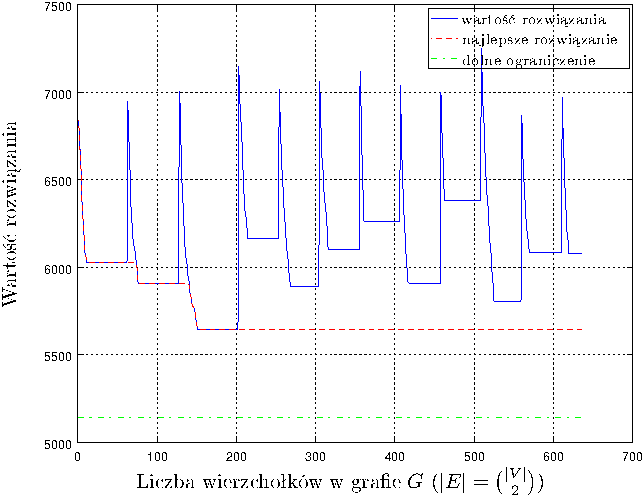
\includegraphics[width=\textwidth]{Chapter_VI/RRIMST5-example/RRIMST5_psfrag}
		\caption{}
		\label{fig:rrimst2:a}
	\end{subfigure}
	\hfill
	\begin{subfigure}[b]{0.32\textwidth}
		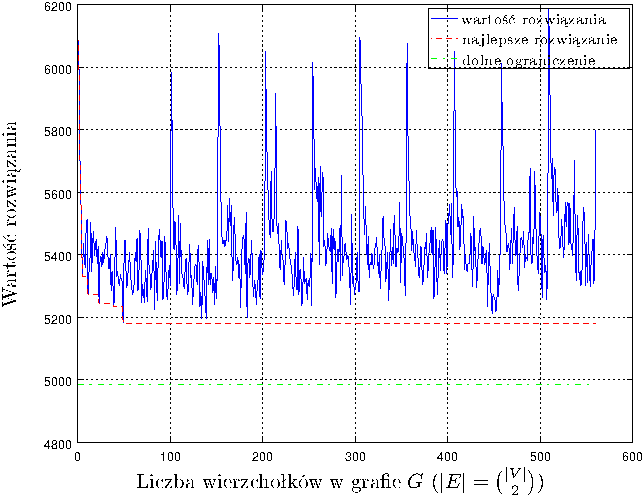
\includegraphics[width=\textwidth]{Chapter_VI/RRIMST6-example/RRIMST6_psfrag}
		\caption{}
		\label{fig:rrimst2:b}
	\end{subfigure}
	\hfill
	\begin{subfigure}[b]{0.32\textwidth}
		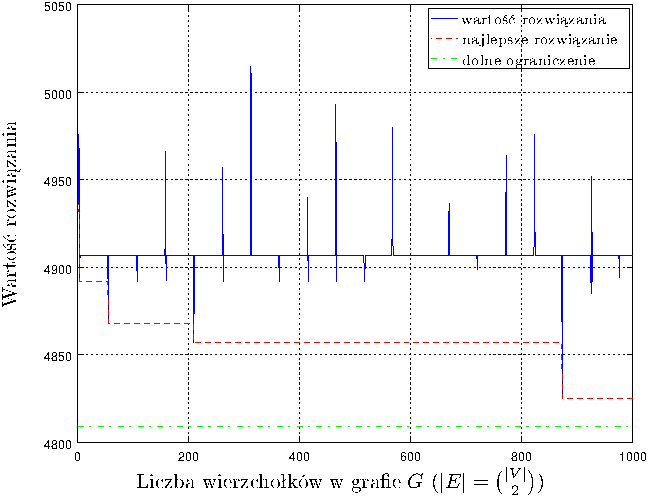
\includegraphics[width=\textwidth]{Chapter_VI/RRIMST7-example/RRIMST7_psfrag}
		\caption{}
		\label{fig:rrimst2:c}
	\end{subfigure}
	\hfill\null
	\caption{
		Wartości rozwiązań zwracane przez algorytm \textsc{Tabu Search} dla grafu o~$30$ wierzchołkach, $435$ krawędziach (gęstość grafu $q = 1$), dla współczynników funkcji oceny ruchu (patrz \ref{eq:moveValue}): $\alpha_{1} = \frac{1}{10}$, $\alpha_{2} = \alpha_{3} = \alpha_{4} = \alpha_{5} = \frac{1}{5}$, dla różnych wartości parametru $k$.
		Długość każdej iteracji dla wszystkich trzech wykresów wynosi $50$.
		Wykresy przedstawiają przebieg algorytmu dla
		\textbf{(a)}~$k = 1$, 
		\textbf{(b)}~$k = 7$,
		\textbf{(c)}~$k = 25$, gdzie krawędzi w~minimalnym drzewie rozpinającym jest $29$.
	}
	\label{fig:rrimst2}
\end{figure}

Widzimy wyraźnie zależności, które występują między poszczególnymi rozwiązaniami.
W~przypadku gdy $k = 1$, otrzymujemy sytuację bardzo podobną do tej, którą przedstawiały wykresy od \ref{fig:rrimst1:a} do \ref{fig:rrimst1:d}~--- tym razem jednak takie zachowanie się algorytmu \textsc{Tabu Search} jest podyktowane bardzo niewielkimi możliwościami wpływania na rozwiązanie pomiędzy kolejnymi jego krokami, gdzie w~każdej iteracji możliwa jest tylko zamiana jednej krawędzi.
Z~uwzględnieniem listy ruchów zakazanych, prowadzi to do tego, że algorytm może ,,poruszać się'' w~bardzo ograniczonym zakresie i~jedyne, co nie jest mu zabronione, to wybieranie z~iteracji na iterację coraz to lepszych rozwiązań, czego przejawem jest właśnie wykres \ref{fig:rrimst2:a}.
Z~drugiej zaś strony widzimy, że poprzez wybranie zbyt dużej wartości $k$ w~stosunku do liczby wierzchołków w~grafie, powodujemy, że algorytm \textsc{Tabu Search} natychmiast zaczyna produkować te same rozwiązania, jako że praktycznie nie są one ograniczone parametrem $k$.
Na tym przykładzie doskonale widać sytuacje, w~której to losowe rozwiązanie (wygenerowane w~momencie przekroczenia dopuszczalnej liczby iteracji) okazuje się być lepsze od najlepszego dotąd znalezionego, gdzie zarówno na wykresie \ref{fig:rrimst2:a} jak i~\ref{fig:rrimst2:b} mamy do czynienia z~taką sytuacją w~bardziej naturalny sposób, gdzie polepszenia wartości rozwiązania występują w~trakcie trwania obliczeń, w~ramach dopuszczalnej liczby iteracji (choć i~tu możemy dostrzec specyficzne zachowania, gdzie przez dość długi okres na wykresie \ref{fig:rrimst2:a} widzimy, że odnajdywane co iteracje rozwiązania są lepsze od swoich poprzedników~--- można wręcz powiedzieć, że wykres \ref{fig:rrimst2:a} w~bardzo wyraźny sposób przedstawia główną ideę algorytmu \textsc{Tabu Search}, pomimo że zastosowany dla $k = 1$ zachowuje się pomiędzy ,,restartami'' jak algorytm zachłanny).
Na samym końcu mamy wykres \ref{fig:rrimst2:b}, którego sposób zachowania świadczy o~poprawnym dobraniu stosunków wszystkich współczynników algorytmu dla tak zadanych danych. 

Choć wszystkie trzy wykresy mają tylko charakter poglądowy, mają przedstawiać różnice, jakie można uzyskać w~działaniu prezentowanego algorytmu, możemy dla wszystkich trzech podać miarę ich efektywności, za jaką będziemy przyjmować procent, o~jaki zbliżyliśmy się do wartości dolnego ograniczenia w~stosunku do początkowego rozwiązania (zobacz tabele od \ref{fig:rrimst2tab:a} do \ref{fig:rrimst2tab:c}) w~czasie działania algorytmu.
Jak możemy zaobserwować, dla wielu różnych konfiguracji algorytm potrafi sobie radzić z~zadanym problemem bardzo różnie, zazwyczaj nie zwracając gorszej odpowiedzi niż $10\%$ od największego dolnego ograniczenia\footnote{
	Największe z~dolnych ograniczeń nie jest wyznacznikiem, mówiącym jak daleko dane rozwiązanie jest oddalone od rozwiązania optymalnego w~rzeczywistości~--- pokazuje jedynie największą możliwą różnice między tymi dwoma rozwiązaniami, jako że to optymalne znajduje się gdzieś pomiędzy nimi.
}.
Na koniec przyglądniemy się jeszcze czterem wykresom, gdzie każdy z~nich przedstawia przebieg algorytmu \textsc{Tabu Search} dla problemu \textsc{Recoverable Robust Incremental Minimum Spanning Tree}, dla pełnego grafu o~$30$ wierzchołkach.
Dla każdej z~instancji problemu zastosowaliśmy różne, opisane pod odpowiednimi wykresami, parametry algorytmu \textsc{Tabu Search}, otrzymując dla niektórych z~nich wartości rozwiązań, których odległość od dolnego ograniczenia na wartość optymalną nie przekracza $1\%$.
Szczególnie wartym zauważenia jest sytuacja, którą uchwyciliśmy na wykresie \ref{fig:rrimst4:a}, gdzie po ponad $500$ iteracjach zostało znalezione takie rozwiązanie, którego wartość okazała się przybliżyć nas do optymalnego rozwiązania z~$0,78\%$ do $0,19\%$.
Pokazuje to jak bardzo nieprzewidywalną może okazać się stosowana przez nas heurystyka i~jak trudnym zadaniem jest eksperymentalne dobieranie jej wszystkich współczynników tak, aby otrzymywane rozwiązania były jak najlepsze.

\begin{table}[!htbp]
	\caption{
		Tabele przedstawiające odległości znajdowanych rozwiązań od dolnych ograniczeń, wyliczonych dla konkretnych instancji problemu. 
		Kolejno w~tabeli są przedstawione: numer iteracji algorytmu \textsc{Tabu Search}, dla której prezentowana jest aktualnie najlepsza, znaleziona do tej pory wartość rozwiązania zadanego problemu oraz wyrażenie, pokazujące procentowo odległość tej wartości od dolnego ograniczenia.
		 \textbf{(a)}~Miejsca, w~których na wykresie \ref{fig:rrimst2:a} możemy obserwować poprawę najlepszego znalezionego rozwiązania. 
		 W~ciągu $151$ iteracji algorytmu zwracane rozwiązanie zostało poprawione o~nieco ponad $23\%$ w~stosunku do rozwiązania początkowego i~znajduje się co najwyżej o $9,74\%$ od rozwiązania optymalnego.
		 \textbf{(b)}~Te same dane przedstawione zostały dla wykresu \ref{fig:rrimst2:b}
		 \textbf{(c)}~oraz \ref{fig:rrimst2:c}.
	}
	\label{fig:rrimst2tab}
	\null\hfill
	\begin{subtable}[b]{0.3\textwidth}
		\centering
		\begin{tabular}{ccc}
			\hline
			\# & $v_{\textsc{ts}} \left( T, S \right)$ & $\frac{v_{\textsc{ts}} \left( T, S \right) - v_{\textsc{ts}}^{LB^{\ast}}}{v_{\textsc{ts}}^{LB^{\ast}}}$ \\
			$1$	&	$6837$	&	$32,91\%$ \\
			$5$	&	$6389$	&	$24,20\%$ \\
			$9$	&	$6082$	&	$18,23\%$ \\
			$73$	&	$6030$	&	$17,22\%$ \\
			$76$	&	$5907$	&	$14,83\%$ \\
			$141$	&	$5869$	&	$14,09\%$ \\
			$145$	&	$5776$	&	$12,29\%$ \\
			$151$	&	$5645$	&	$9,74\%$ \\\hline                                                                                                    
		\end{tabular}
		\caption{}
		\label{fig:rrimst2tab:a}
	\end{subtable}
	\hfill
	\begin{subtable}[b]{0.3\textwidth}
		\centering
		\begin{tabular}{ccc}
			\hline
			\# & $v_{\textsc{ts}} \left( T, S \right)$ & $\frac{v_{\textsc{ts}} \left( T, S \right) - v_{\textsc{ts}}^{LB^{\ast}}}{v_{\textsc{ts}}^{LB^{\ast}}}$ \\
			$1$	&	$6086$	&	$22,11\%$	\\
			$2$	&	$5731$	&	$14,99\%$	\\
			$4$	&	$5452$	&	$9,39\%$	\\
			$5$	&	$5331$	&	$6,96\%$	\\
			$11$	&	$5274$	&	$5,82\%$	\\
			$23$	&	$5243$	&	$5,20\%$	\\
			$39$	&	$5234$	&	$5,02\%$	\\
			$49$	&	$5182$	&	$3,97\%$	\\\hline                                                                                                  
		\end{tabular}
		\caption{}
		\label{fig:rrimst2tab:b}
	\end{subtable}
	\hfill
	\begin{subtable}[b]{0.3\textwidth}
		\centering
		\begin{tabular}{ccc}
			\hline
			\# & $v_{\textsc{ts}} \left( T, S \right)$ & $\frac{v_{\textsc{ts}} \left( T, S \right) - v_{\textsc{ts}}^{LB^{\ast}}}{v_{\textsc{ts}}^{LB^{\ast}}}$ \\
			$1$	&	$4936$	&	$2,64$\%	\\
			$2$	&	$4936$	&	$2,64$\%	\\
			$3$	&	$4892$	&	$1,73$\%	\\
			$54$	&	$4892$	&	$1,73$\%	\\
			$55$	&	$4868$	&	$1,23$\%	\\
			$209$	&	$4857$	&	$1,00$\%	\\
			$210$	&	$4857$	&	$1,00$\%	\\
			$873$	&	$4825$	&	$0,33$\%	\\\hline                                                                                                     
		\end{tabular}
		\caption{}
		\label{fig:rrimst2tab:c}
	\end{subtable}
	\hfill\null
\end{table}

\begin{figure}[!h]
	\renewcommand\figurename{Wykres}
	\null\hfill
	\begin{subfigure}[b]{0.45\textwidth}
		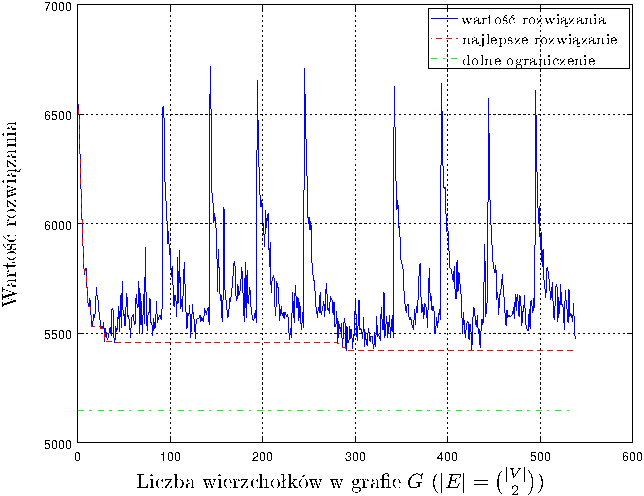
\includegraphics[width=\textwidth]{Chapter_VI/RRIMST8-example/RRIMST8_psfrag}
		\caption{}
		\label{fig:rrimst3:a}
	\end{subfigure}
	\hfill
	\begin{subfigure}[b]{0.45\textwidth}
		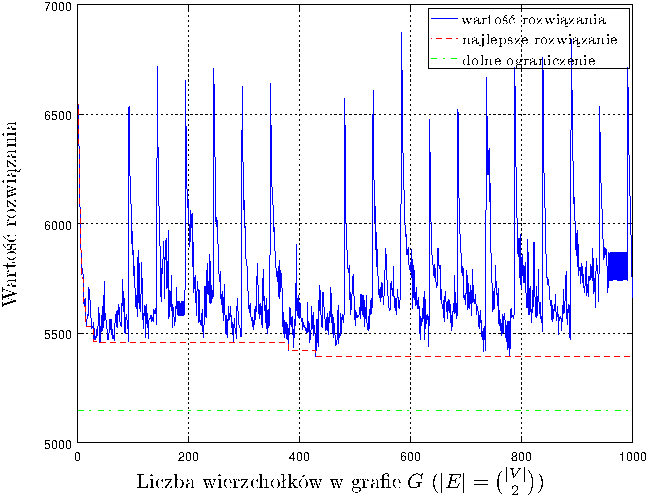
\includegraphics[width=\textwidth]{Chapter_VI/RRIMST9-example/RRIMST9_psfrag}
		\caption{}
		\label{fig:rrimst3:b}
	\end{subfigure}
	\hfill\null
	\caption{
		Wartości rozwiązań zwracane przez algorytm \textsc{Tabu Search} dla grafu o~$30$ wierzchołkach, $435$ krawędziach (gęstość grafu $q = 1$), dla parametru $k = 3$ oraz maksymalną liczbą iteracji wynoszącą $50$.
		 \textbf{(a)}~Przebieg algorytmu \textsc{Tabu Search} dla współczynników funkcji oceny ruchu $\alpha_{1} = \frac{1}{10}$, $\alpha_{2} = \alpha_{3} = \alpha_{4} = \alpha_{5} = \frac{1}{5}$.
		 Na przestrzeni $290$ iteracji, w~czasie których algorytm $4$ razy rozpoczynał poszukiwanie rozwiązania w~innym punkcie przestrzeni rozwiązań, początkowe rozwiązanie zdołano poprawić o~nieco ponad $20\%$ (zobacz tabelę \ref{fig:rrimst3tab:a}).
		 \textbf{(b)}~Przebieg algorytmu dla tej samej instancji problemu ze zmienionymi współczynnikami funkcji oceny ruchu: $\alpha_{1} = \frac{1}{5}$, $\alpha_{2} = \alpha_{3} = \alpha_{4} = \alpha_{5} = \frac{4}{5}$.
		 W~tym przypadku, tak jak to widać w~tabelach \ref{fig:rrimst3tab:a} oraz \ref{fig:rrimst3tab:b}, zmiana sposobu podejmowania decyzji odnośnie następnych ruchów pozwoliła jeszcze bardziej zbliżyć się do optymalnego rozwiązania dla problemu.
	}
	\label{fig:rrimst3}
\end{figure}

\begin{table}[!htbp]
	\caption{
		Tabele przedstawiające odległości znajdowanych rozwiązań od dolnych ograniczeń, wyliczonych dla instancji problemów, które zostały przedstawione na wykresach:
		\textbf{(a)}~\ref{fig:rrimst3:a} oraz
		\textbf{(b)}~\ref{fig:rrimst3:b}.
	}
	\label{fig:rrimst3tab}
	\null\hfill
	\begin{subtable}[b]{0.3\textwidth}
		\centering
		\begin{tabular}{ccc}
			\hline
			\# & $v_{\textsc{ts}} \left( T, S \right)$ & $\frac{v_{\textsc{ts}} \left( T, S \right) - v_{\textsc{ts}}^{LB^{\ast}}}{v_{\textsc{ts}}^{LB^{\ast}}}$ \\
			$1$	&	$6546$	&	$27,26\%$	\\
			$3$	&	$6227$	&	$21,05\%$	\\
			$9$	&	$5768$	&	$12,13\%$	\\
			$13$	&	$5622$	&	$9,29\%$	\\
			$25$	&	$5519$	&	$7,29\%$	\\
			$40$	&	$5455$	&	$6,05\%$	\\
			$281$	&	$5450$	&	$5,95\%$	\\
			$290$	&	$5420$	&	$5,37\%$ \\\hline                                                                                                    
		\end{tabular}
		\caption{}
		\label{fig:rrimst3tab:a}
	\end{subtable}
	\hfill
	\begin{subtable}[b]{0.3\textwidth}
		\centering
		\begin{tabular}{ccc}
			\hline
			\# & $v_{\textsc{ts}} \left( T, S \right)$ & $\frac{v_{\textsc{ts}} \left( T, S \right) - v_{\textsc{ts}}^{LB^{\ast}}}{v_{\textsc{ts}}^{LB^{\ast}}}$ \\
			$1$	&	$6546$	&	$27,26\%$	\\
			$4$	&	$6059$	&	$17,79\%$	\\
			$9$	&	$5768$	&	$12,13\%$	\\
			$15$	&	$5530$	&	$7,50\%$	\\
			$25$	&	$5519$	&	$7,29\%$	\\
			$40$	&	$5455$	&	$6,05\%$	\\
			$380$	&	$5420$	&	$5,37\%$	\\
			$429$	&	$5391$	&	$4,80\%$	\\\hline                                                                                                  
		\end{tabular}
		\caption{}
		\label{fig:rrimst3tab:b}
	\end{subtable}
	\hfill\null
\end{table}

\begin{figure}[!h]
	\renewcommand\figurename{Wykres}
	\null\hfill
	\begin{subfigure}[b]{0.45\textwidth}
		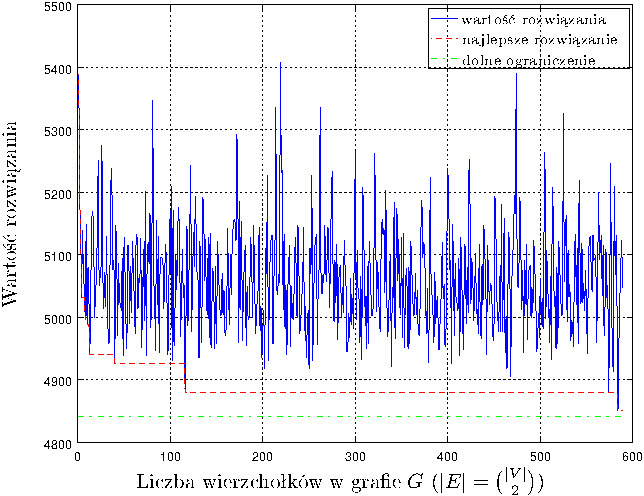
\includegraphics[width=\textwidth]{Chapter_VI/RRIMST10-example/RRIMST10_psfrag}
		\caption{}
		\label{fig:rrimst4:a}
	\end{subfigure}
	\hfill
	\begin{subfigure}[b]{0.45\textwidth}
		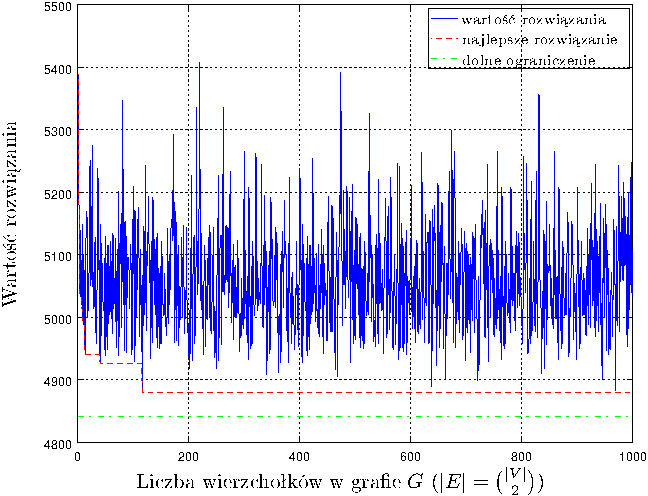
\includegraphics[width=\textwidth]{Chapter_VI/RRIMST11-example/RRIMST11_psfrag}
		\caption{}
		\label{fig:rrimst4:b}
	\end{subfigure}
	\hfill\null
	\caption{
		Wartości rozwiązań zwracane przez algorytm \textsc{Tabu Search} dla grafu o~$30$ wierzchołkach, $435$ krawędziach (gęstość grafu $q = 1$), dla parametru $k = 15$ oraz maksymalną liczbą iteracji wynoszącą $50$.
		 \textbf{(a)}~Przebieg algorytmu \textsc{Tabu Search} dla współczynników funkcji oceny ruchu identycznych jak dla wykresu \ref{fig:rrimst3:a}: $\alpha_{1} = \frac{1}{10}$, $\alpha_{2} = \alpha_{3} = \alpha_{4} = \alpha_{5} = \frac{1}{5}$.
		 Na przestrzeni prawie $600$ iteracji początkowe rozwiązanie zdołano poprawić o~nieco ponad $11\%$, osiągając tym samym niemal wartość dolnego ograniczenia.
		 \textbf{(b)}~Przebieg algorytmu dla tej samej instancji problemu ze zmienionymi współczynnikami funkcji oceny ruchu: $\alpha_{1} = \frac{1}{5}$, $\alpha_{2} = \alpha_{3} = \alpha_{4} = \alpha_{5} = \frac{4}{5}$.
		 Odwrotnie niż to miało miejsce na wykresach \ref{fig:rrimst3:a} oraz \ref{fig:rrimst3:a}, w~tym przypadku zmiana parametrów funkcji oceny ruchu, pomimo zwiększenia ogólnej liczby iteracji, nie przyniosła oczekiwanych rezultatów w~postaci polepszenia rozwiązania (zobacz tabele \ref{fig:rrimst4tab:a} oraz \ref{fig:rrimst4tab:b}).
	}
	\label{fig:rrimst4}
\end{figure}

\begin{table}[!h]
	\caption{
		Tabele przedstawiające odległości znajdowanych rozwiązań od dolnych ograniczeń, wyliczonych dla instancji problemów, które zostały przedstawione na wykresach:
		\textbf{(a)}~\ref{fig:rrimst4:a} oraz
		\textbf{(b)}~\ref{fig:rrimst4:b}.
	}
	\label{fig:rrimst4tab}
	\null\hfill
	\begin{subtable}[b]{0.3\textwidth}
		\centering
		\begin{tabular}{ccc}
			\hline
			\# & $v_{\textsc{ts}} \left( T, S \right)$ & $\frac{v_{\textsc{ts}} \left( T, S \right) - v_{\textsc{ts}}^{LB^{\ast}}}{v_{\textsc{ts}}^{LB^{\ast}}}$ \\
			$1$	&	$5388$	&	$11,28\%$	\\
			$3$	&	$5151$	&	$6,38\%$	\\
			$8$	&	$4996$	&	$3,18\%$	\\
			$10$	&	$4988$	&	$3,02\%$	\\
			$13$	&	$4941$	&	$2,04\%$	\\
			$40$	&	$4927$	&	$1,76\%$	\\
			$116$	&	$4880$	&	$0,78\%$	\\
			$584$	&	$4851$	&	$0,19\%$ \\\hline                                                                                                    
		\end{tabular}
		\caption{}
		\label{fig:rrimst4tab:a}
	\end{subtable}
	\hfill
	\begin{subtable}[b]{0.3\textwidth}
		\centering
		\begin{tabular}{ccc}
			\hline
			\# & $v_{\textsc{ts}} \left( T, S \right)$ & $\frac{v_{\textsc{ts}} \left( T, S \right) - v_{\textsc{ts}}^{LB^{\ast}}}{v_{\textsc{ts}}^{LB^{\ast}}}$ \\
			$1$	&	$5388$	&	$11,28\%$	\\
			$3$	&	$5151$	&	$6,38\%$	\\
			$4$	&	$5032$	&	$3,92\%$	\\
			$8$	&	$4996$	&	$3,18\%$	\\
			$10$	&	$4988$	&	$3,02\%$	\\
			$13$	&	$4941$	&	$2,04\%$	\\
			$40$	&	$4927$	&	$1,76\%$	\\
			$116$	&	$4880$	&	$0,78\%$	\\\hline                                                                                                  
		\end{tabular}
		\caption{}
		\label{fig:rrimst4tab:b}
	\end{subtable}
	\hfill\null
\end{table}